\section{Introduction}
\begin{frame}
	\frametitle{Basic 'Mesh' Terminology}
  \begin{itemize}
		\item \keyword{Mesh Generation} (\keyword{Meshing}) is the act of creating a mesh for a computing task
		\item Generally a \keyword{Mesh} is a discretized representation of a geometry 
		\item Meshes are used in FEM, FV, FD, Physics Simulators (Rigid or Soft Bodies), CAD, Rendering, 3D Printing,...
		\item Mesh Generation software is often specialized for a certain target application ($\uparrow$)
		\item Larger software packages often have mesh generation software included as a component of the package
		\item Meshes used for computational tasks need to fulfill certain \keyword{quality criteria}
		\item \keyword{Quality criteria} are checked before use to prevent unnecessary failure and remeshing
		\item \keyword{Mesh Data Structures}, \keyword{Mesh Formats} and \keyword{Mesh Conversion} are essential components of the meshing workflow
  \end{itemize}	
\end{frame}

\begin{frame}
	\frametitle{Mesh Generation}
  \begin{itemize}
		\item Mesh Generation is a huge/important aspect of simulation (for mesh-based methods of course)
		\item Manual, automatic and hybrid (combination of manual + automatic) mesh generation methods
		\item Computational domains have different components that can be meshed differently
		\item Meshing of inflow, outflow, wall, embedded geometry or other special function components of the domain
		\item Surface meshes (usually surface triangulations) are frequently used to simulate flow around objects
		\item Create a mesh that fulfills the quality criteria for the designated computation task
		\item Involves scientific disciplines such as computational geometry, differential geometry, geometric modeling, optimization, etc.
  \end{itemize}	
\end{frame}

\begin{frame}
	\frametitle{Mesh Nomenclature}
  \begin{itemize}
		\item Focus on 2D Meshes, 3D Surface/Volume meshes
		\item Basic topological terminology and theory of meshes in the works of Kinsey \cite{kinsey1993topology} and 
Edelsbrunner\cite{Edelsbrunner:2006:GTM:1137760}.		
  \end{itemize}		
  \begin{block}{Definition: Mesh or Cell Complex}
  A mesh $\mathcal M$ is composed of a finite number of $n$-dimensional cells: 
	\begin{align*}
   \mathcal M =\{\omega : \omega \text{ is a element}\}.  
  \end{align*}
  \end{block}	
  \begin{itemize}
		\item \keyword{Cell Complex} is a common alternative term for mesh in literature
		\item Term is used computational geometry package \keyword{CGAL} and implemented as a data structure
  \end{itemize}			
\end{frame}

\begin{frame}
  \frametitle{Cell Complex Example}
	\begin{block}{Hexahedron Example}
   The hexahedron is composed of one 3-dimensional element/cell, the 3-dimensional cell is composed of six 2-dimensional cells, the facets. The facets are
	 composed of the 1-cells called edges/segments describing their boundaries. The endpoints of the edges are the eight 0-dimensional cells, the vertices.
	\end{block}
    \begin{center}
      \includegraphics[width=0.4\textwidth]{screenshots/hexa-cell2.png}
    \end{center}			
\end{frame}

\begin{frame}
  \frametitle{Dimension of a Cell Complex}
 	\begin{block}{Dimension of a Cell Complex}
	The dimension of a mesh is equal to the highest cell dimension in the mesh.
   A cell of a mesh is the mesh component the inner of which is homeomorphic to the inner set of an $n$-dimensional disk.  
	\end{block}
  \begin{itemize}
		\item The boundary of a cell is composed of cells of lower dimension, these lower dimensional cell boundaries are
 called \keyword{faces} or \keyword{facets}.
		\item For these relationship between faces and cells we can also use the notation $\sigma < \tau$ to indicate that $\sigma$ is a face of cell $\tau$.
		\item A polyhedron for example is a cell that is composed of polygonal faces(two-dimensional cells), edges (one-dimensional cells) and vertices (zero-dimensional cells).
  \end{itemize}	
\end{frame}

\begin{frame}
  \frametitle{Structure of a Cell Complex}
In order to construct a mesh we combine and connect cells of equal dimension: vertices are connected to vertices and edges are connected to \keyword{adjacent} edges. 
 	\begin{block}{Dimension of a Cell Complex}
By $|\mathcal M|$ we refer to the set of points of mesh $\mathcal M$:	
\begin{align*}
  |\mathcal M|=\{\vec{x} : \vec{x} \in \sigma \in \mathcal M, \text{$\sigma$ is a cell in $\mathcal M$.}\}  
\end{align*}
	\end{block}
  \begin{itemize}
		\item $|\mathcal M|$ is also called the underlying space of $\mathcal M$
		\item For every vertex in $|\mathcal M|$ a defined neighborhood relationship has to exist
		\item Neighborhood in a 2-cell complex:
		\begin{itemize}
			\item Vertex neighborhoods over edge connections
			\item Facet neighborhood over edges			
			\item Facet neighborhood over vertices
			\item ...									
		\end{itemize}				
  \end{itemize}		
\end{frame}

\begin{frame}
  \frametitle{Neighborhoods/Connectivity in a Cell Complex}
		\begin{itemize}
			\item For vertex $\vec{v}$ inside of a polygon, the neighborhood of $\vec{v}$ is an arbitrary disk that is entirely located in the inside 
of the polygon. 
			\item If the vertex $\vec{v}$ is on an edge $\vec{e}$ that was contructed by unification of edges $\vec{e}_0,\dots,\vec{e}_n$ then the corresponding vertex $\vec{v}$ has to be present on every edge $\vec{e}_i$.
			\item Facet neighborhood over vertices
			\item The unification of half-disk neighborhoods of the vertices $\vec{v}_0,\dots,\vec{v}_n$ leads to the neighbor relationship that is
depicted in figure \ref{fig:mesh-neighborhood}.
			\item When $\vec{v}$ is contructed from polygon vertices $\vec{v}_0,\dots,\vec{v}_n$ the neighborhood of $\vec{v}$ is composed of the different disc- or half-disc neighborhoods of $\vec{v}_0,\dots, \vec{v}_n$.  
		\end{itemize}					 
\begin{figure}[h!]
\begin{center}
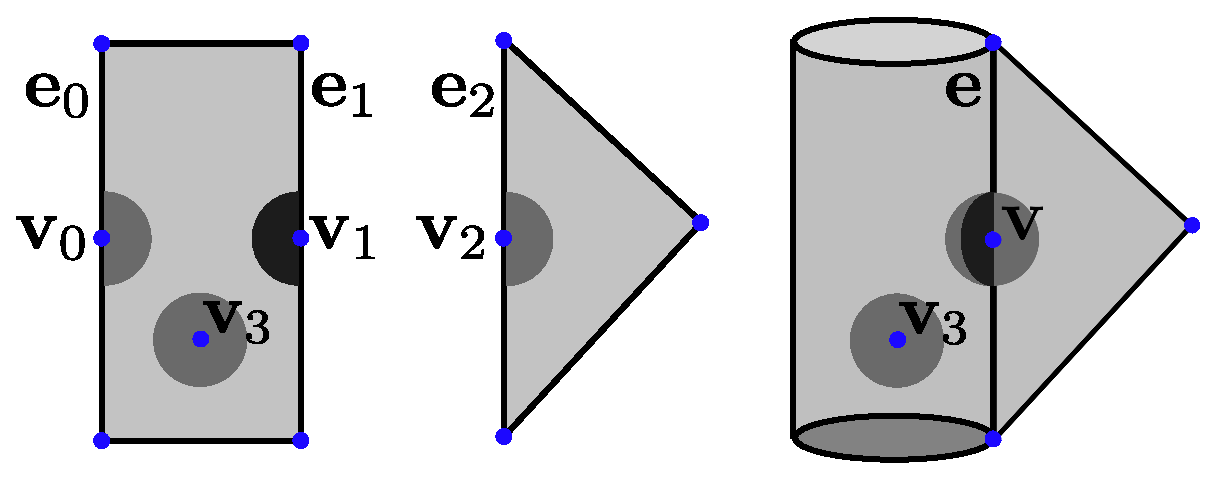
\includegraphics[height=3cm]{screenshots/neighborhood.eps}
\end{center}
\caption{We unify edges $\vec{e}_0$, $\vec{e}_1$ and $\vec{e}_2$, the resulting cell complex or mesh is on the right. The vertex $\vec{v}$ that has been produced by
unifying the other vertices also has a neighborhood that is the result of the unification of $\vec{v}_0$, $\vec{v}_1$ and $\vec{v}_2$ \cite{kinsey1993topology}.}
\label{fig:mesh-neighborhood}
\end{figure}

\end{frame}

\begin{frame}
  \frametitle{Adjacency, Incidence, Valency and Stencil}
From basic graph theory the adjacency and incidency relationships are important for our
considerations:
		\begin{itemize}
			\item \keyword{Adjacency} is the neighborhood relation between same type mesh components whereas \keyword{incidency} is the neighborhood relation between mesh components of
a different type.
			\item Using this terminology we call two polygons adjacent if there is an edge that is incident to both polygons
							 
 
\item The \keyword{stencil} of a vertex is the set of edges and polygons incident to the vertex:
\begin{align*}
  Stencil \text{ } \tau = \{\sigma \in K| \tau < \sigma \}
\end{align*}
\item The \keyword{degree} or \keyword{valency} of a vertex $\vec{v}$ is the number of vertices $\vec{v}_i$ that is adjacent to $\vec{v}$, meaning there exists an edge that connects $\vec{v}$ to $\vec{v}_i$.
\end{itemize}
\end{frame}

\begin{frame}
  \frametitle{Surface Meshes}
\begin{itemize}
\item Usually a triangulation or quadrangulation of a geometric object
\item In CFD simulations used as:
	\begin{itemize}
	  \item Domain boundaries
	  \item Immersed static objects		
	  \item Immersed dynamic objects				
	\end{itemize}
\item Immersion of surface meshes into CFD simulations usually done by \keyword{Fictitious Domain} Methods (FEATFLOW: \keyword{Fictitious Boundary})
\end{itemize}
\begin{figure}[h!]
\centering
\subfloat[Streamline flowfield around a \newline helix geometry]{ 
 \includegraphics[height=3cm]{Images/helix.eps}
 \label{fig:helix}
}%\hspace{0.1cm}
\subfloat[ Twin screw geometry simulation ]{ 
 \includegraphics[height=3cm]{Images/liquidsolid_intro.eps}
 \label{fig:liquidsolid_intro}
}
\caption{CFD Examples with surface meshes}
\label{fig:liquid-solid}
\end{figure}
\end{frame}

\begin{frame}
\frametitle{Surface Meshes Example}

\begin{figure}[h!]
	\begin{center}
	   \includegraphics[width=\textwidth]{screenshots/tori.jpg}
	\end{center}
	%\caption{From left to right: manifold surface, non-manifold at an edge and non-manifold at a vertex.}
	\label{fig:tori}
\end{figure}
\end{frame}

\begin{frame}
For multiple tasks surfaces are required to be \keyword{manifolds}:
\begin{itemize}
\item An $n$-dimensional manifold is a topological space in which every vertex has a neighborhood that is topologically equivalent to an open $n$-dimensional disk. 
\item Two distinct points have disjoint neighborhoods, a surface is a \keyword{2-manifold} 
\item If a manifold has a boundary then there exist vertices that have a neighborhood that is topologically equivalent to an open $n$-dimensional disk or half-disk
\item If a vertex has neither an open disk nor open half-disk neighborhood then it is called \keyword{non-manifold}
\item If a surface has one or more non-manifold vertices then the surface is called a non-manifold surface
\end{itemize}
\begin{figure}[h!]
\begin{center}
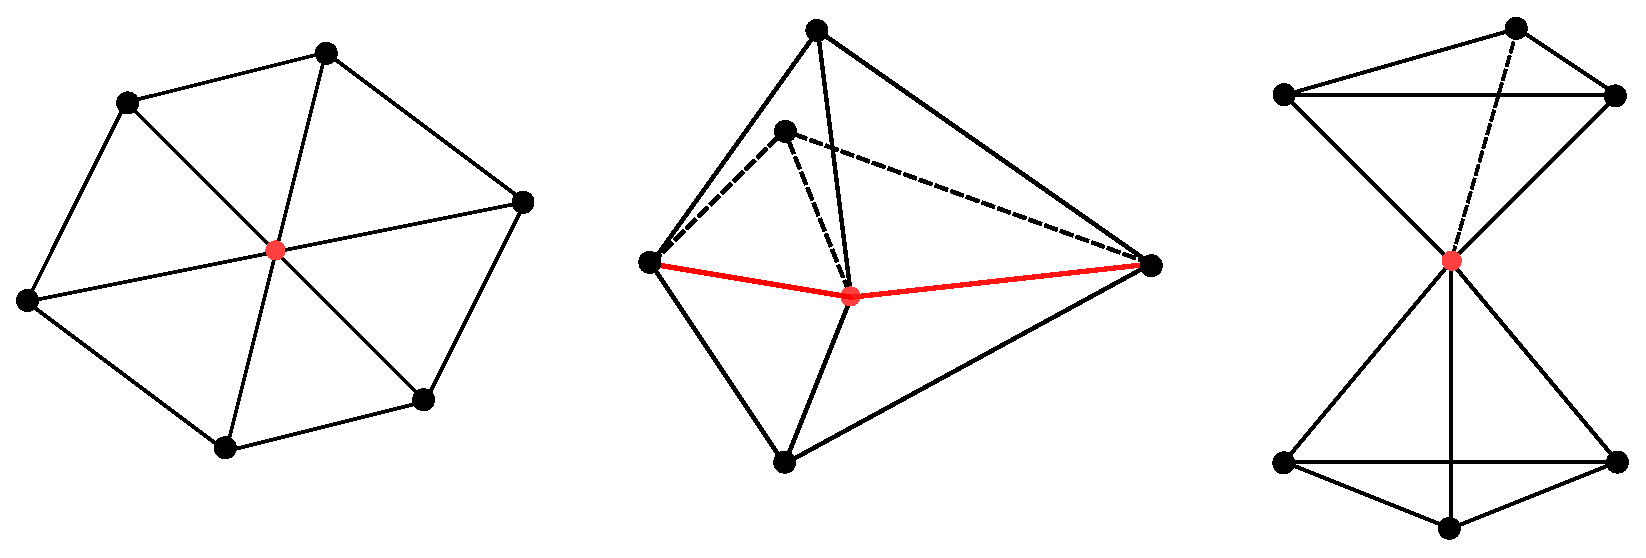
\includegraphics[height=3cm]{screenshots/non_manifolds.eps}
\end{center}
\caption{From left to right: manifold surface, non-manifold at an edge and non-manifold at a vertex.}
\label{fig:non-manifold}
\end{figure}
\end{frame}

\begin{frame}
A bounded manifold can be either \keyword{orientable} or \keyword{non-orientable}
\begin{itemize}
\item A surface is orientable if it does not contain a \keyword{Moebius Strip} \cite{Edelsbrunner:2006:GTM:1137760}.
\item A Moebius Strip can be explained by considering an $(n+1)$-dimensional object moving continiously along an n-manifold
\item If the the object is located on one side of the n-manifold and on its travelling path it revisits a neighborhood, but this time from the other side, then this path is a Moebius Strip and the surface is not orientable
\item The surfaces used to construct two-dimensional meshes are orientable, the cells of these meshes are triangles or quadrilaterals, which are connected by vertices or edges
\item Thus, there should be no isolated vertices or edges that are not part of a polygon in our mesh according to this terminology
\end{itemize}

\begin{figure}[h!]
 \includegraphics[height=3cm]{screenshots/moebius.jpg}
 \label{fig:moebius-render}
\caption{A Moebius Strip can be created by twisting and connecting the edges of a planar strip, see also \cite{Edelsbrunner:2006:GTM:1137760,kinsey1993topology}.}
\label{fig:moebius}
\end{figure}
\end{frame}

\begin{frame}
\frametitle{Software For Generation and Processing of Surface Meshes}

\begin{itemize}
	\item \keyword{Blender}: Creation, manipulation, format conversion, visualization, analysis, postprocessing, open-source, Python scripting
	\item \keyword{Autodesk 3DS Max}: As Blender, but commercial, a bit more advanced manipulation features, proprietary scripting language, Windows only
	\item \keyword{Meshlab}: Mesh analysis, correction of mesh defects, calculation of various mesh properties and indicators
	\item \keyword{Autodesk Inventor}: CAD, creation of meshes from \keyword{NURBS}-Surfaces \cite{NURBSBOOK}
	\item \keyword{FreeCAD}: Open-source CAD program, less functions than Inventor
	\item \keyword{CGAL}: Open-source modern C++ software library for creation, manipulation, analysis, geometric algorithms,...
	\item \keyword{OpenMesh}: Open-source modern C++ data structure for surface meshes from RWTHA 	
\end{itemize}

\end{frame}

\begin{frame}{Data Formats for Surface Meshes}
    \begin{columns}
        \column{0.5\textwidth}{
            \begin{exampleblock}{Element-List}
                \begin{itemize}
                  \item STL
                \end{itemize}
								Properties
                \begin{itemize}
                  \item Stores each element and vertex coordinates
                  \item Redundant repetition of coordinates									
                  \item Problem: Vertex coordinates may not coincide $\rightarrow$ invalid mesh										
                  \item Can store additional properties									
                  \item Main usage for graphics renderings									
                \end{itemize}								
            \end{exampleblock}       }
        \column{0.5\textwidth}{
            \begin{alertblock}{Connectivity-Based}
                \begin{itemize}
                  \item Wavefront OBJ		
                  \item OFF
                  \item Stanford PLY
                  \item VTK									
                \end{itemize}
								Properties:
                \begin{itemize}
                  \item List of vertices, followed by list of elements with vertex indices
									\item more storage efficient
                  \item Some formats allow to store additional properties
                \end{itemize}								
            \end{alertblock}       }
    \end{columns}
\end{frame}

\begin{frame}
\frametitle{OpenMesh - A Surface Mesh Data Structure}
\begin{itemize}
\item \url{https://www.graphics.rwth-aachen.de/software/openmesh/}
\item Uses the efficient halfedge (or winged edge) to the mesh and the connectivity
\item Iterators allow the user to iterate through vertices, edges, faces
\item Circulators allow the user to:
\begin{itemize}
\item iterate over all neighboring vertices of a vertex
\item iterate over all incident edges of a vertex
\item iterate over all faces attached to a vertex
\item iterate over a face's vertices
\item iterate over the face's incident edges
\item iterate over the adjacent faces
\end{itemize}
\item Store user-defined traits in vertices, edges, halfedges, faces	
\end{itemize}								
\end{frame}

\begin{frame}
\frametitle{OpenMesh - The Halfedge Data Structure}
\begin{figure}[h!]
 \includegraphics[width=0.8\textwidth]{screenshots/half-edge.png}
\caption{The OpenMesh Half-Edge Data Structure \cite{Botsch02openmesh}.}
\end{figure}
\end{frame}

\begin{frame}
\frametitle{Software For Generation and Processing of Surface Meshes}
The process of generating meshes that are well suited for using them in a numerical simulation is 
called \textit{mesh generation} and can be called a scientific discipline on its own right. The use of meshes is necessitated by the fact that the partial differential equations,
that describe the physical phenomena that we want to simulate can be solved analytically only for very basic cases on simple domains. In order to solve realistic
problems the domain needs to be discretized by a computational mesh so that the system of equations can be discretized. Some of the most popular mesh-based numerical 
solution techniques for PDEs include the Finite Volume method, the Finite Difference method and the Finite-Element method. The reason why we have briefly summarized 
the very basic foundation of meshes and their topology is that it allows us to formally introduce structured and unstructured meshes. In the remainder of this 
introduction to computational meshes we will examine structured and unstructured meshes and discuss their properties. In a numerical simulation the choice of mesh 
type and element type is dependent on the numerical simulation scheme and the concrete problem that needs to be solved. Not only the type of mesh employed is problem-dependent,
but also the generation of the topological mesh structure depends on the type of physical problem and its specific features, the compute hardware that is 
available, the desired accuracy of the result, the available compute time 
and findings from previous simulations with different meshes.
\end{frame}

\begin{frame}
A structured mesh is characterized by the feature that the degree vertices, the number of vertices adjacent to a mesh vertex, is the same throughout the
whole mesh or in other words that it has a regular connectivity (with the exception of boundary vertices). The storage of such a mesh in computer memory can be realized by a simple array 
of cells. This most simple
type of storage is discouraged in case the mesh is to refined in the course of the application, because new vertices need to be inserted which makes additional
storage of connectivity information neccessary. Usual choices of elements in a structured mesh include quadrilateral elements in 2D and hexahedral elements in 3D. 
Elements like tetrahedrons are in general not used in structured meshes. The reason for this is that tetrahedrons require more elements to fill a domain with elements.
The advantages of tetrahedrons, their ability to represent complex geometries better, do not play a significant role in structured meshes. As the 
approach in structured meshes to approximate geometries better is by additional refinement levels while keeping the mesh structure simple which is easier to do
with regular hexahedral elements. 
\end{frame}

\begin{frame}
There exist different subtypes of structured meshes that are used as computational meshes which mainly include equidistant cartesian meshes, rectilinear and curvilinear meshes these are
illustrated in figure \ref{fig:structured}. 
The equidistant cartesian meshes have many advantageous properties: they have a uniform element size and it is possible to easily locate an arbitrary point in the mesh, that is a relation between
a location in space and an element can be established easily. For rectilinear and curvilinear meshes establishing this relation is also possible, but slightly more difficult. 
In terms of memory representation of such meshes this means that an element index in a data structure
can be efficiently computed based on coordinates in space:
\begin{equation}
  \vec{p} \mapsto i\text{ (array index) }, \vec{p} \in \mathbb{R}^3.
  \label{eq:struct-map}
\end{equation}
Equidistant cartesian meshes are often used for parallel finite volume, finite difference or 
general high performance computing schemes because of their easy generation, memory access patterns and simple domain decomposition capabilities. Besides their use in 
these applications equidistant structured meshes are used as acceleration structures for geometric computations where there are employed as a means to subdivide space.
These properties make equidistant cartesian meshes and variants popular choices for spatial subdivision structures intended for acceleration of geometric 
calculations or other application specific geometric queries (visibility determination, point containment, distance or intersection queries).
\end{frame}

\begin{frame}
\begin{figure}[h!]
\centering
\subfloat[Equidistant cartesian mesh]{ 
 \includegraphics[height=3cm]{Images/equidistant.eps}
 \label{fig:equidistant}
}\hspace{0.2cm}
\subfloat[Rectilinear mesh]{ 
 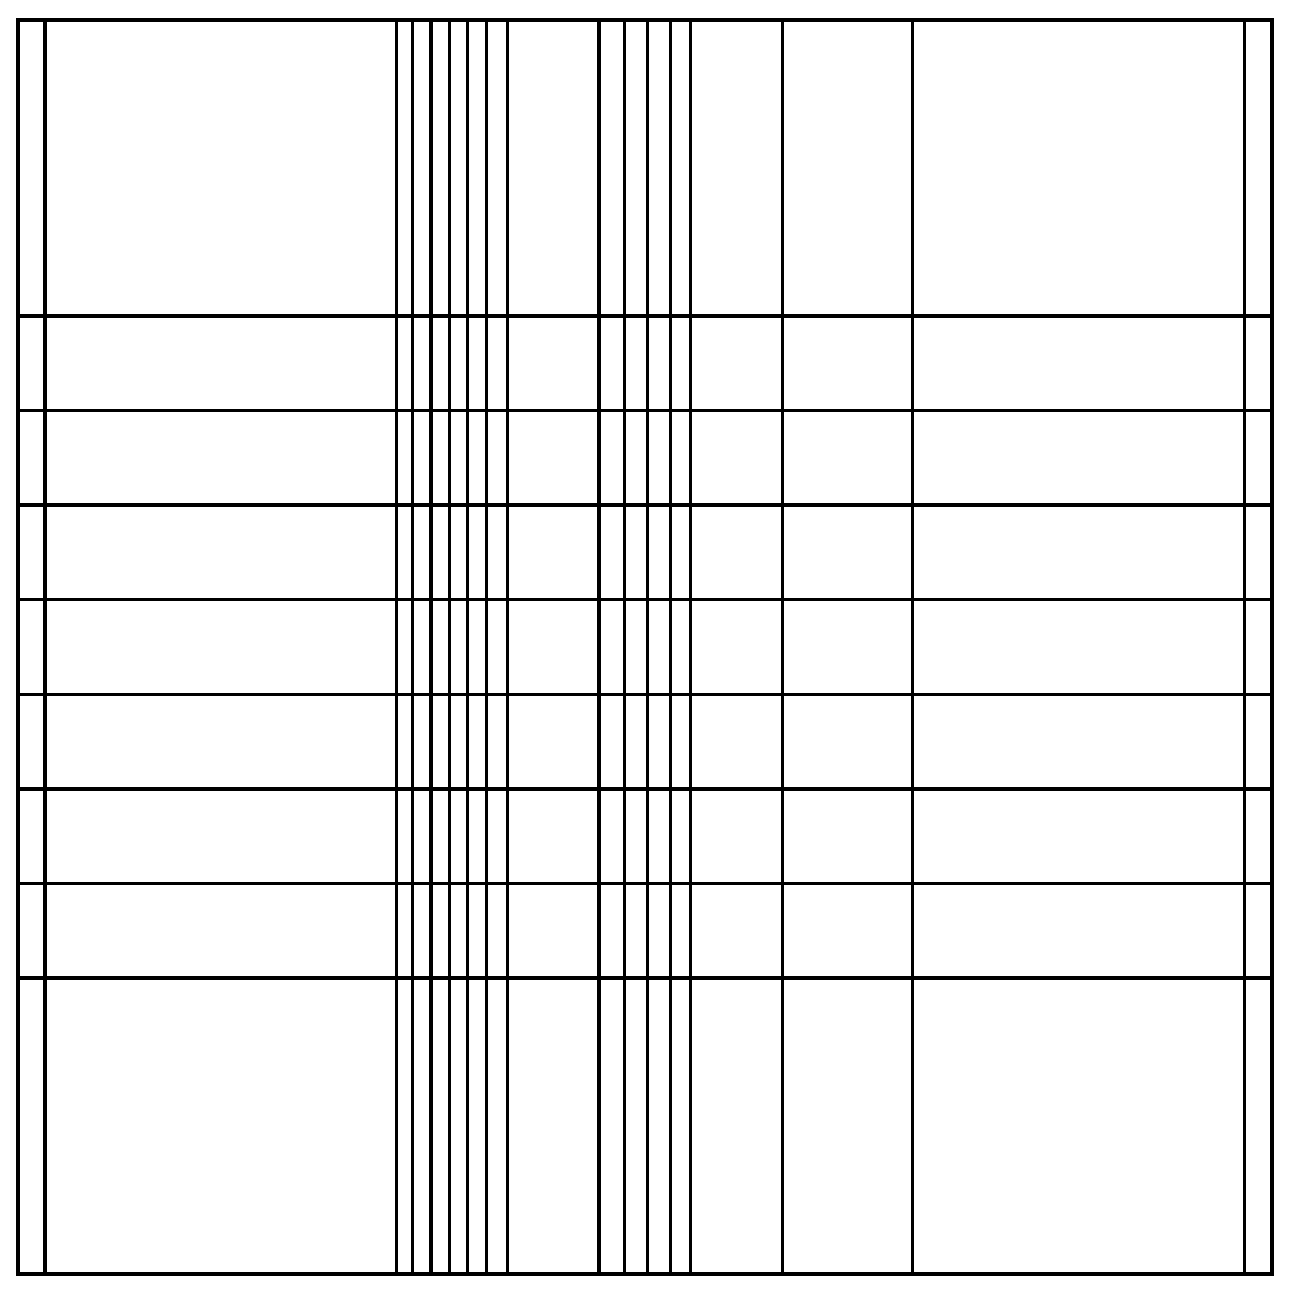
\includegraphics[height=3cm]{Images/rectilinear.eps}
 \label{fig:rectilinear}
}\hspace{0.2cm}
\subfloat[Curvilinear mesh]{ 
 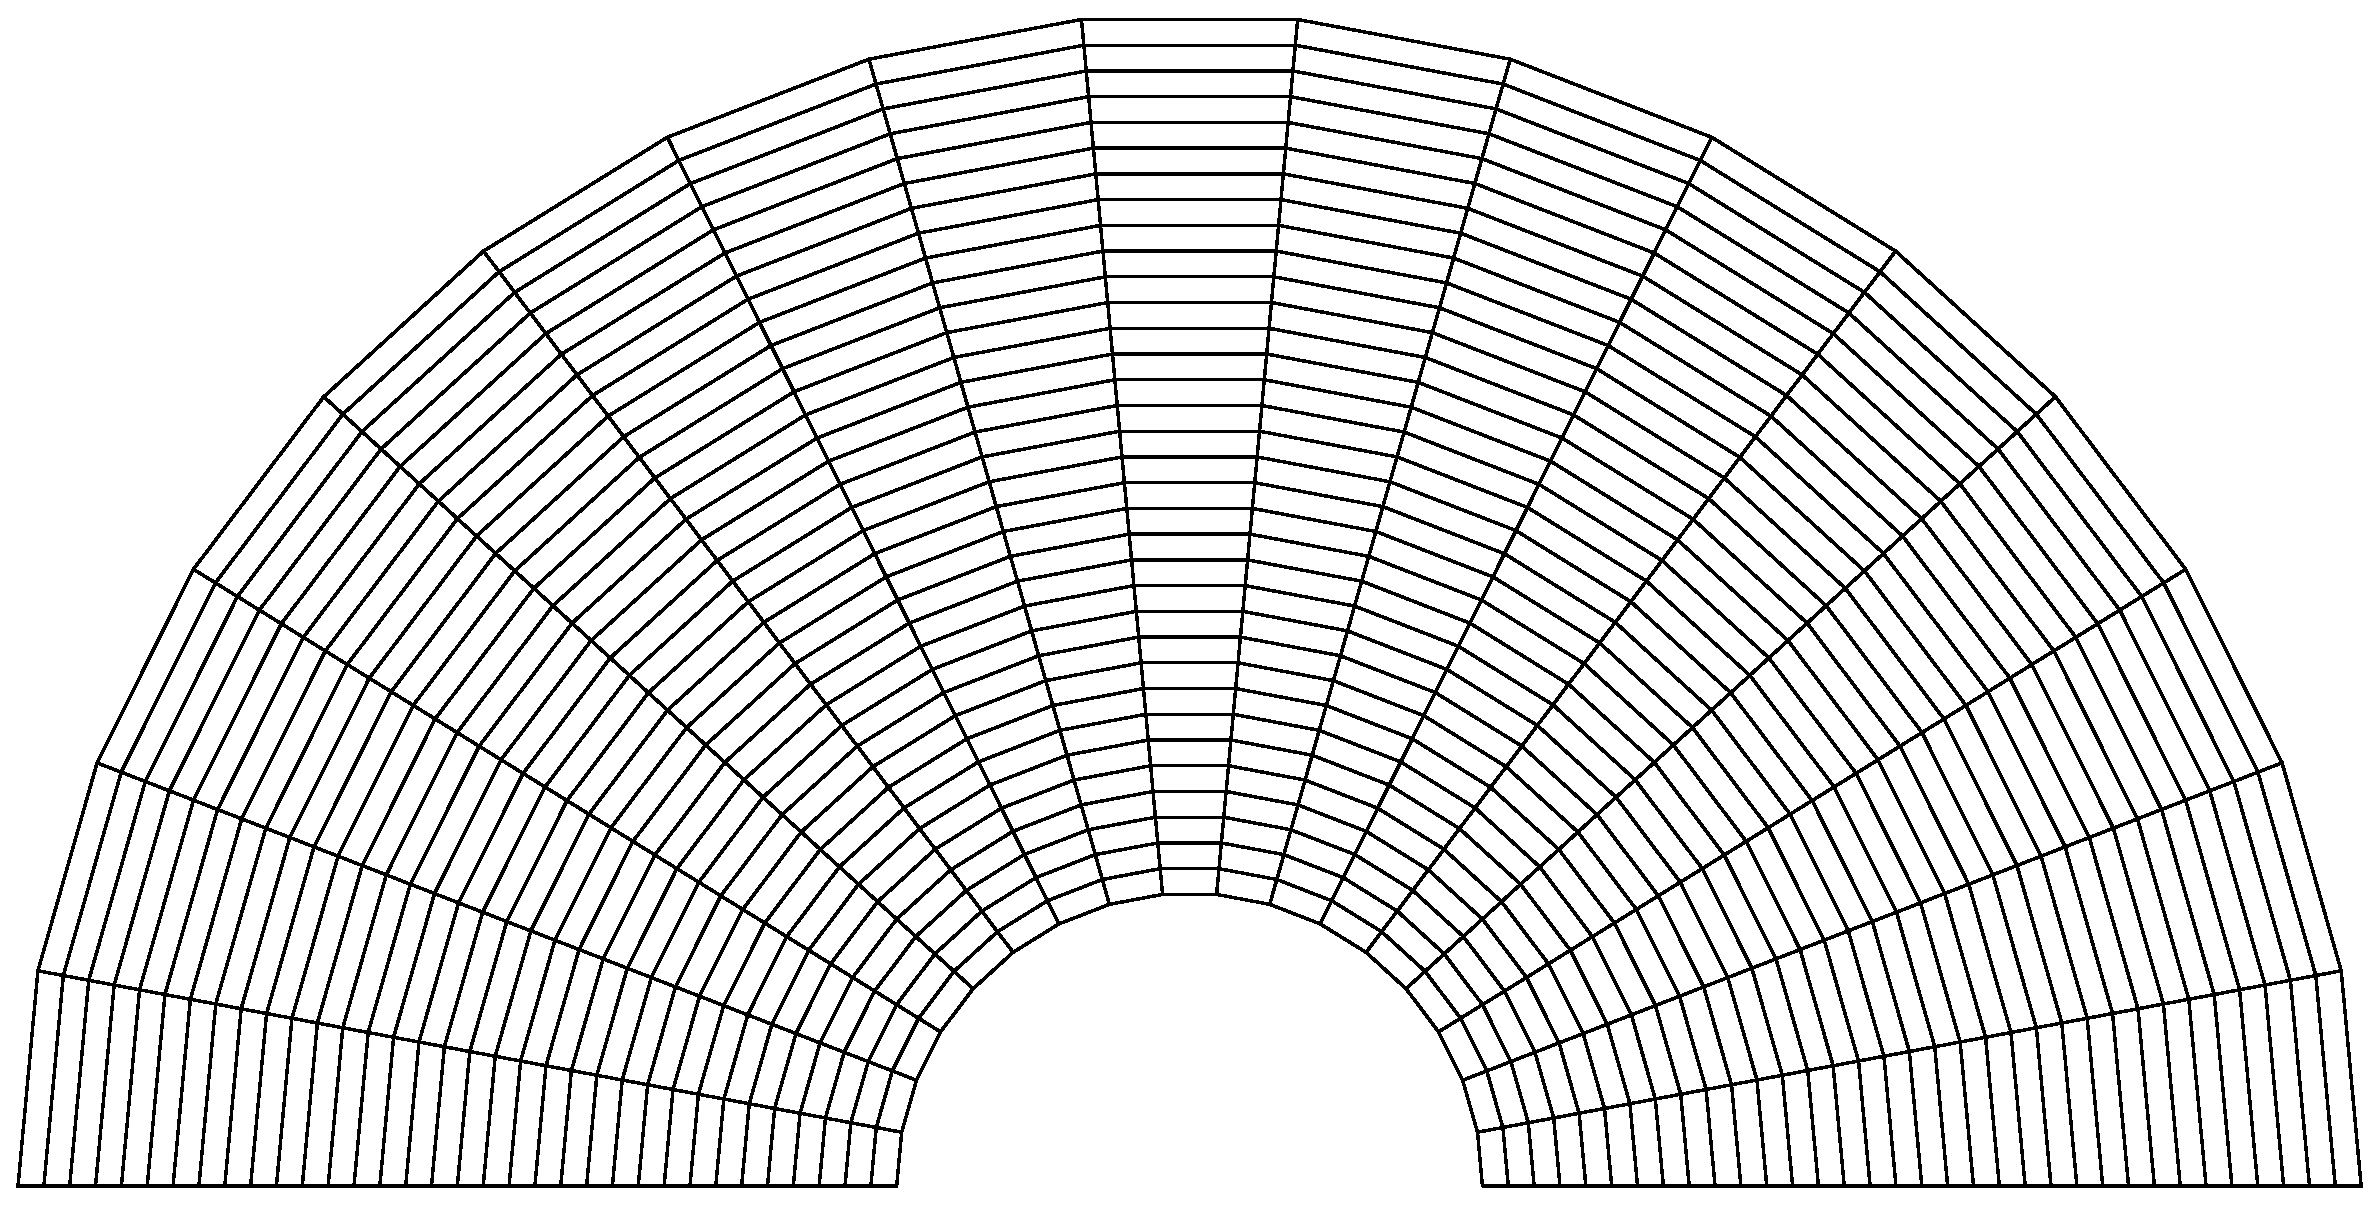
\includegraphics[height=3cm]{Images/curvilinear.eps}
 \label{fig:curvilinear}
}
\caption{Structured meshes used as computational meshes, from left to right: equidistant structured mesh, rectilinear mesh and curvilinear mesh.}
\label{fig:structured}
\end{figure}
\end{frame}

\begin{frame}
In an unstructured mesh the vertices in general do not have a predefined uniform vertex degree. In principle this means that an arbitrary number of cells can be
incident to a vertex. The freedom of not being confined to a uniform vertex valency allows for better geometry resolution by the mesh, which is especially
helpful in the case of complex geometries. Furthermore, unstructured meshes can employ connector elements to gradually reduce the level of refinement in a grid
from domain areas where a high mesh resolution is required to domain areas where such a high mesh resolution is not needed (see figure \ref{fig:unstructured-fac}). This property is a clear advantage over
structured meshes where the mesh resolution can only be increased globally or by local vertex redistribution without changing the 
connectivity of the mesh. The choice of unstructured meshes in order to better approximate complex-shaped geometries introduces some difficulties as well. Complex 
geometries are often explicitly defined by a set of coordinates in space or by an explicit or implicit analytic function. Using an unstructured mesh there is 
in general no easy way to introduce a mapping from positions in space to element indices in computer memory. Which means that calculations that involve geometric 
information about the object that is represented by the mesh may need to resort to exhaustive search procedures if no measure are taken to add this feature to the 
class of unstructured meshes. Possible solutions to this problem are discussed in the following chapters. Standard choices for cell geometries in unstructured meshes are hexahedrons, tetrahedrons or prisms.\\
\begin{figure}[h!]
\begin{center}
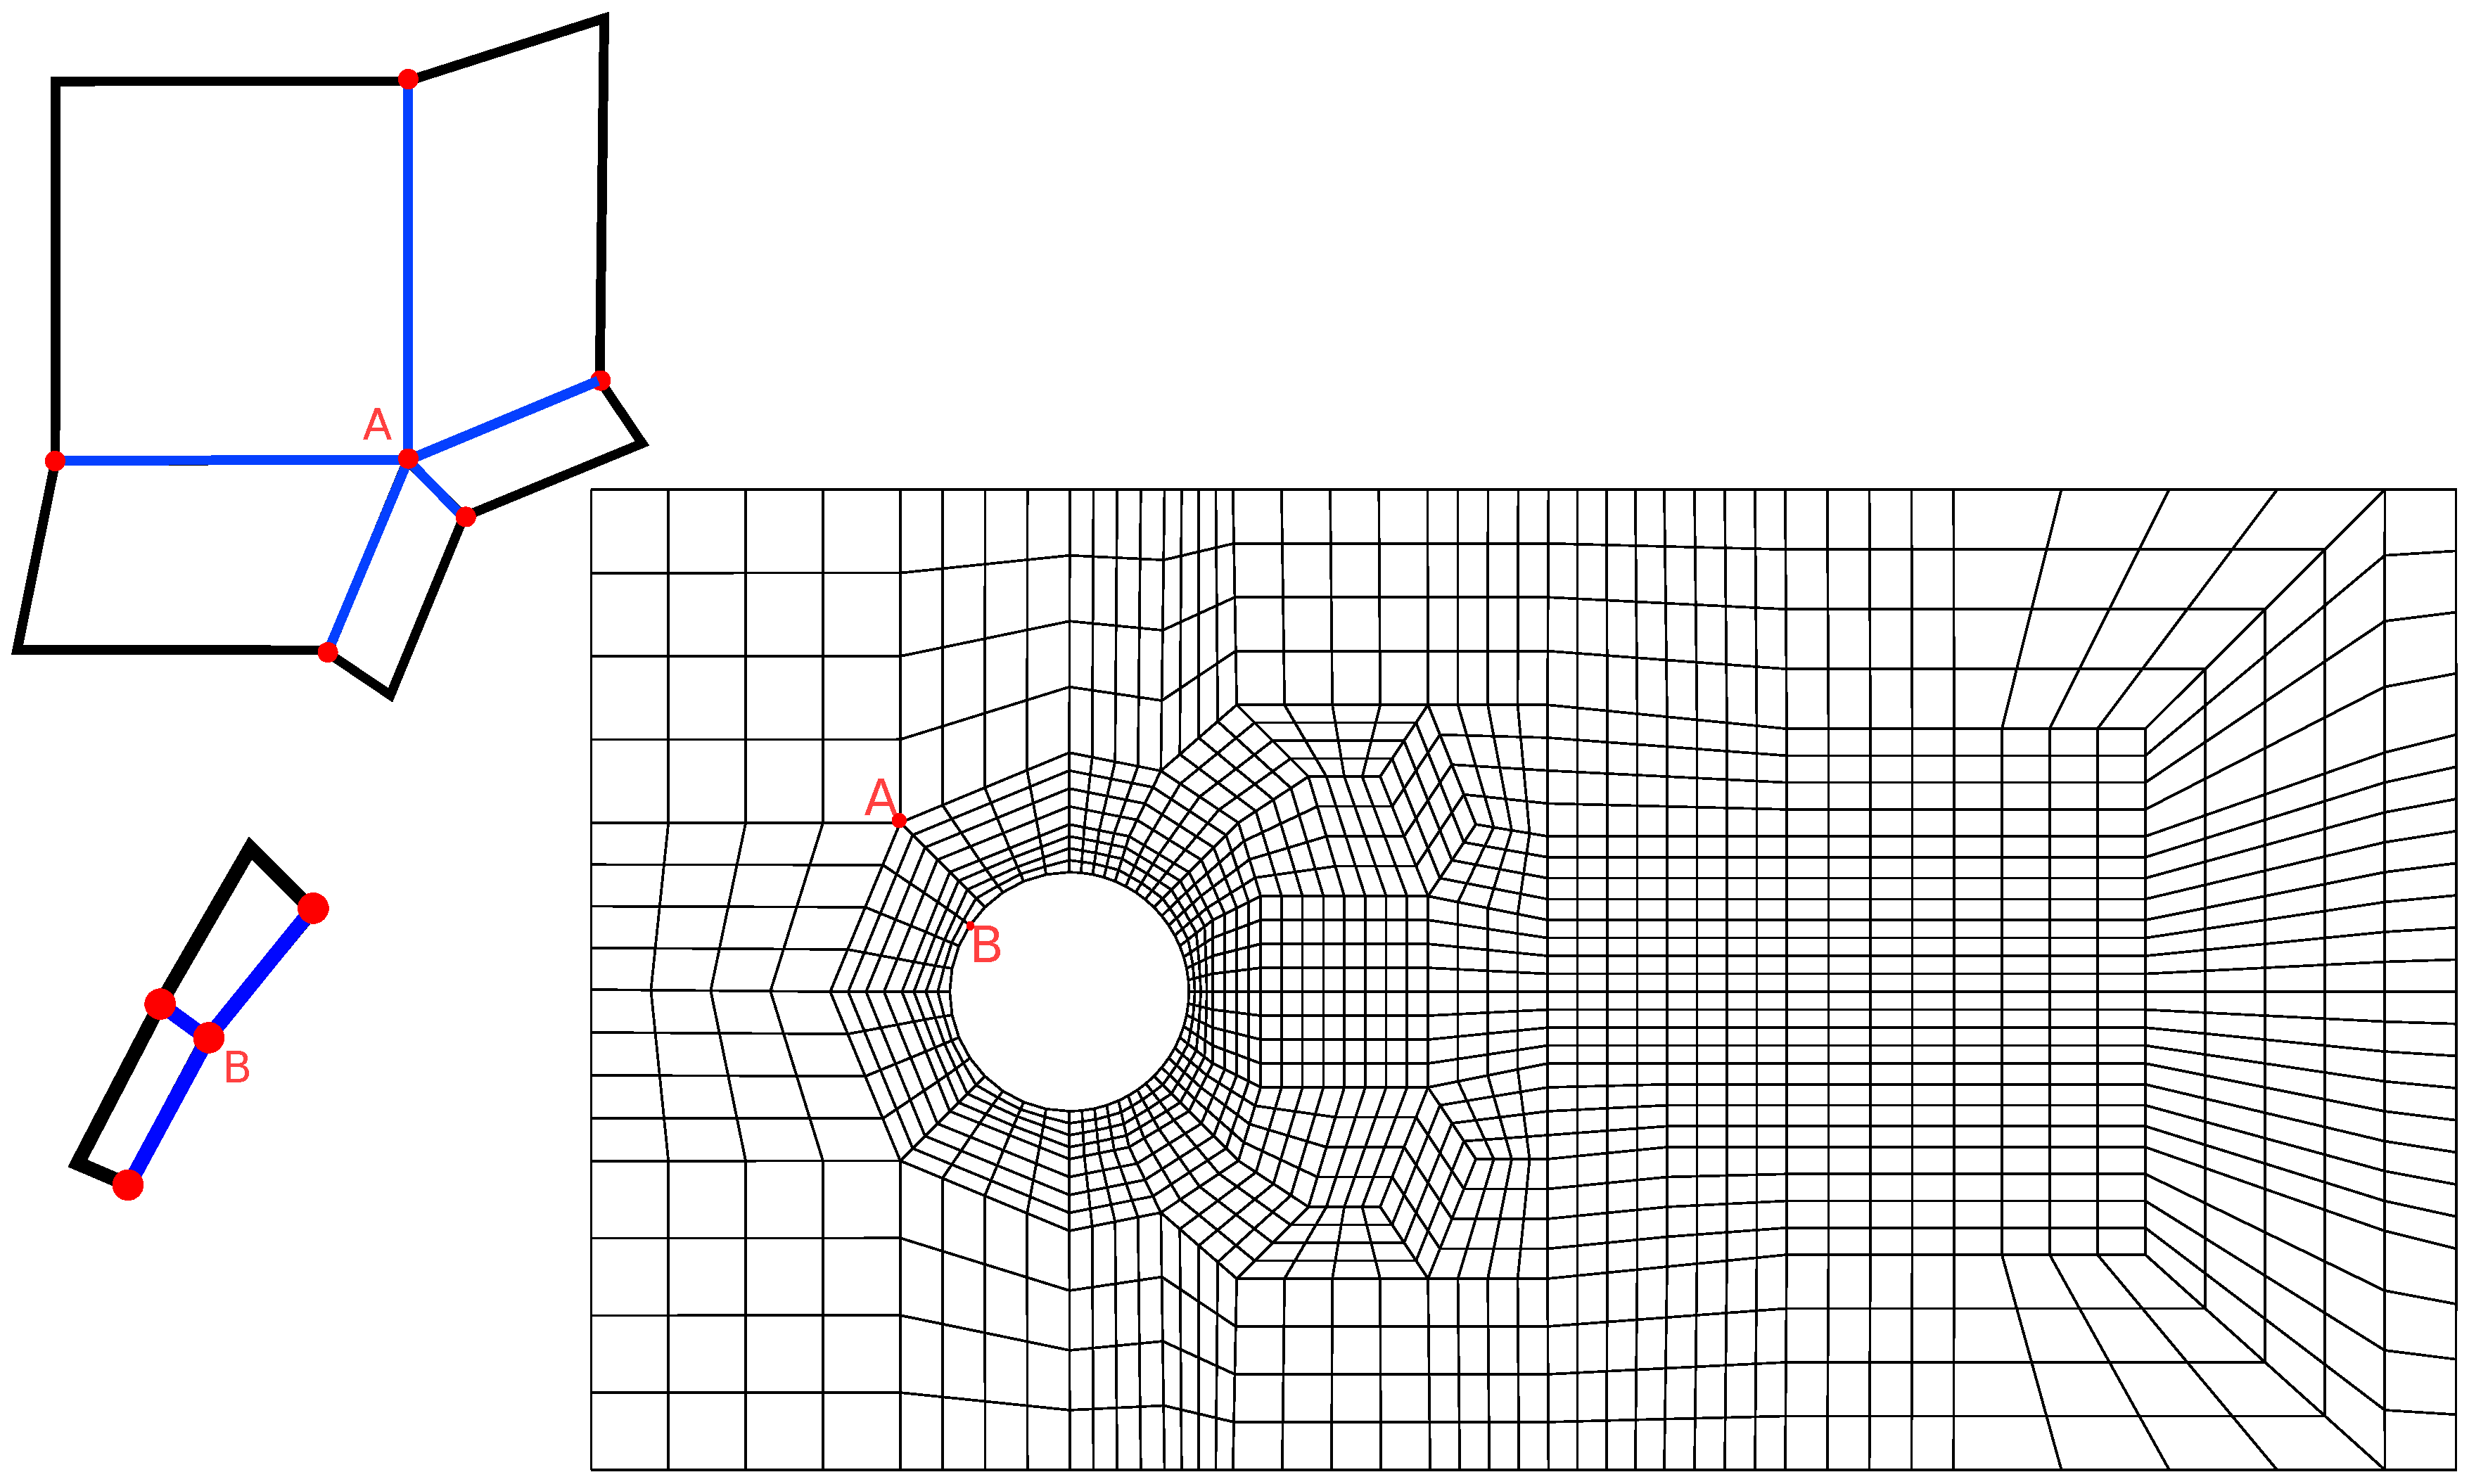
\includegraphics[height=7cm]{Images/fac_unstructured.eps}
\end{center}
\caption{Unstructured 2D mesh where the mesh edges are aligned with an inner circle. We have marked some vertices with different 
degrees to that are used as anchor for connector elements (A) or as elements that approximate the circle geometry with its edges (B).}
\label{fig:unstructured-fac}
\end{figure}
\end{frame}

\begin{frame}
open volume mesh
salome
gitter adaptivität
\end{frame}